\documentclass[11pt]{article}

% --- Style (loads geometry, amsmath, lineno, fancyhdr, authblk, etc.) ---
\usepackage{bioarxiv}

% --- Figures and tables ---
\usepackage{graphicx}
\graphicspath{{figures/}}
\usepackage{booktabs}

% --- Bibliography ---
\usepackage[numbers,sort&compress]{natbib}

% --- Subfigures ---
\usepackage{subcaption}

% --- Smart references (MUST load after hyperref, which is in bioarxiv.sty) ---
\usepackage{cleveref}

% ====================================================================
% METADATA
% ====================================================================
\runningtitle{Evo2 zero-shot VEP for spaceflight genes}
\leadauthor{Kim \textit{et al.}}

\title{Evo2 zero-shot variant effect prediction across 215,001 coding
       and non-coding variants in spaceflight radiation-response genes}

\author[1]{JangKeun Kim}
\author[1,2]{Christopher E.\ Mason\,\orcidlink{0000-0002-1850-1642}}
\affil[1]{Department of Physiology and Biophysics, Weill Cornell Medicine,
          New York, NY 10065, USA}
\affil[2]{The WorldQuant Initiative for Quantitative Prediction,
          Weill Cornell Medicine, New York, NY 10065, USA}

\correspondingauthor{chm2042@med.cornell.edu}

\date{}  % leave empty for preprint

% ====================================================================
\begin{document}

\maketitle
\printcorrespondence

% --- Abstract ---
\begin{abstract}

\textbf{Background:}
Variant effect prediction (VEP) is a bottleneck in clinical variant
interpretation. Existing tools are restricted to specific variant types---missense
(AlphaMissense, REVEL), splice-altering (SpliceAI)---or incorporate clinical
databases in training (CADD), creating potential circularity. No single tool
provides unified, training-data-free predictions across coding, non-coding, and
indel variants. Spaceflight radiation generates characteristic transversion
mutations and complex DNA damage in genes critical for radiation response,
telomere maintenance, and DNA repair, yet comprehensive variant effect maps
for these genes are lacking.

\textbf{Results:}
We applied Evo2, a 7-billion-parameter genomic foundation model trained on 9.3
trillion nucleotides, to score 215,001 variants (168,409 SNVs and 46,592 indels)
across ten spaceflight radiation-response genes in a zero-shot manner requiring
no training data. Deep mutational scanning calibration against four independent
datasets yielded Spearman $|\rho| = 0.21$--$0.52$. ClinVar benchmarking
demonstrated AUROCs of 0.91--1.00 across six genes, with Evo2 achieving the
highest AUROC for CHEK2 (0.9996) and TP53 (0.9887). On matched variant sets,
Evo2 was statistically indistinguishable from CADD (DeLong $p > 0.08$, all
genes). Evo2 scores were orthogonal to supervised tools (Spearman $\rho =
0.41$--$0.83$ vs.\ CADD), and an Evo2+CADD ensemble improved classification
by up to 0.38\%. For non-coding variants, Evo2 was the only tool with a
significant positive correlation with TERT promoter MPRA functional data
($\rho = +0.267$, $p = 3.8 \times 10^{-14}$; CADD, SpliceAI, ncER: not
significant). Frameshift indel AUROCs exceeded 0.94 across six genes (mean
0.977). Transversion-control analysis revealed that the elevated scores for
radiation-signature mutations are attributable to general transversion bias
rather than radiation-specific chemistry.

\textbf{Conclusions:}
Evo2 provides a comprehensive zero-shot variant effect atlas that complements
supervised tools and fills critical gaps for non-coding and indel variants.
The atlas of 215,001 scored variants across ten genes is provided as a
public resource for clinical variant interpretation and astronaut genomic
risk assessment.

\end{abstract}

\keywords{variant effect prediction, genomic foundation model, Evo2, deep
mutational scanning, ClinVar, spaceflight radiation, non-coding variants,
zero-shot prediction, TERT, DNA damage response}


% --- Main text ---
\section{Introduction}
\label{sec:introduction}

The interpretation of genomic variants remains a central bottleneck in clinical
genetics and precision medicine. Despite advances in sequencing technology,
the majority of rare variants detected in human genomes are classified as
variants of uncertain significance (VUS), limiting their clinical
actionability~\cite{ClinVar_2018,ACMG_2015}. Computational variant effect
prediction (VEP) tools provide evidence for the ACMG/AMP PP3 and BP4 criteria,
but each existing tool addresses only a subset of the variant landscape.
AlphaMissense~\cite{AlphaMissense_2023} and REVEL~\cite{REVEL_2016} are
restricted to missense variants; SpliceAI~\cite{SpliceAI_2019} predicts only
splice-altering effects; non-coding scores such as ncER~\cite{ncER_2019} and LINSIGHT~\cite{LINSIGHT_2017}
provide regional constraint estimates but lack variant-level resolution;
and integrative scores such as CADD~\cite{CADD_2024},
though broadly applicable, incorporate ClinVar annotations in their training,
creating potential circularity when used for ClinVar variant
reclassification~\cite{gnomAD_2020}. No single existing tool provides unified,
training-data-free predictions across coding, non-coding, and indel variants.

Genomic foundation models offer a fundamentally different approach. Trained on
large collections of DNA sequences in a self-supervised manner, these models
learn the statistical grammar of genomes without exposure to phenotypic labels.
The Evo family of models---Evo~\cite{Evo1_2024} and
Evo2~\cite{Evo2_2026}---represents the current state of the art in genomic
language modelling, with Evo2's 7-billion-parameter architecture trained on 9.3
trillion nucleotides from 128,000 genomes spanning all domains of life. Evo2
supports context windows up to one million base pairs, far exceeding the Nucleotide
Transformer~\cite{NT_2024} ($\sim$6\,kb effective context) and
HyenaDNA~\cite{HyenaDNA_2023} (450\,kb at reduced resolution). The zero-shot
variant effect prediction paradigm---comparing reference and alternate sequence
log-likelihoods without fine-tuning---enables variant scoring that is intrinsically
free of training-set circularity and agnostic to variant type, including
non-coding and indel variants that remain inaccessible to most supervised tools.

Spaceflight presents a unique context for variant interpretation. Astronauts are
exposed to galactic cosmic radiation (GCR) and solar particle events that
generate characteristic mutational signatures, including C$>$A transversions
from 8-oxoguanine lesions and complex double-strand break (DSB)
repair products~\cite{daSilveira_2020}. The NASA Twins Study revealed persistent
gene expression changes in DNA repair, telomere maintenance, and immune
regulation pathways after long-duration spaceflight~\cite{Twins_2019}, and
Rutter et al.~\cite{Rutter_2024} recently identified protective and risk alleles
in astronaut genomes across genes involved in radiation response. However, the
functional consequences of the vast majority of variants in these genes---particularly
non-coding and structural variants---remain unknown. A comprehensive variant
effect atlas for spaceflight radiation-response genes would support both
mission-planning risk assessment and fundamental understanding of
radiation-induced mutagenesis.

Here we apply Evo2 to generate zero-shot variant effect predictions for 215,001
variants (168,409 SNVs and 46,592 indels) across ten genes selected for their
relevance to spaceflight radiation biology: four well-characterised control genes
(BRCA1, TP53, CHEK2, DNMT3A) with extensive experimental validation data, and
six spaceflight-associated genes (TERT, ATM, NFE2L2, CLOCK, MSTN, RAD51). We
validate predictions through a three-layer framework: (1) deep mutational
scanning (DMS) calibration against four independent functional datasets, (2)
ClinVar clinical benchmarking with multi-tool comparison and matched-variant
analysis, and (3) non-coding validation using TERT promoter MPRA data and ENCODE
regulatory element annotations.

We demonstrate that Evo2 achieves clinical-grade ClinVar AUROCs (0.91--1.00),
is the highest-performing tool for two of six benchmarked genes, provides
orthogonal signal that improves ensemble classification, and---critically---is
the only tool with significant positive correlation with non-coding MPRA data
in the TERT promoter. The resulting variant effect atlas, encompassing coding
and non-coding regions across all ten genes, is provided as a public resource.

\section{Results}
\label{sec:results}

\subsection{Window size optimization identifies 8,192\,\bp{} as optimal}
\label{sec:results_window}

To determine the scoring window that best captures variant context, we evaluated
four window sizes (1,024, 2,048, 4,096, and 8,192\,\bp) on ClinVar-annotated
variants in three well-characterised genes (BRCA1, TP53, CHEK2). The
8,192\,\bp{} window achieved the highest mean AUROC (0.9921) for discriminating
pathogenic from benign variants and was selected for all subsequent analyses
(\Cref{fig:supp_ablation}). Performance improved monotonically with window size
across all three genes, suggesting that flanking-sequence context---including
intronic and regulatory regions---contributes to variant effect prediction.

\subsection{DMS calibration confirms Evo2 captures functional impact}
\label{sec:results_dms}

We calibrated Evo2 $\Delta$LL scores (\Cref{eq:delta_ll}) against deep
mutational scanning data for four control genes (\Cref{fig:dms}A--D). Evo2 showed significant Spearman
correlations with experimentally measured functional scores in all four genes:
BRCA1 ($\rho = +0.515$, $p < 10^{-261}$, $n = 3{,}884$),
DNMT3A ($\rho = +0.457$, $p < 10^{-39}$, $n = 746$),
CHEK2 ($\rho = +0.310$, $p < 10^{-108}$, $n = 4{,}882$),
and TP53 ($\rho = -0.211$, $p < 10^{-29}$, $n = 2{,}827$). The negative
TP53 correlation is expected: the Giacomelli nutlin-3 assay assigns high scores
to loss-of-function variants, inverting the sign convention.

Multi-tool comparison on the same variant sets revealed that Evo2's $|\rho|$
was competitive with supervised tools (\Cref{fig:dms}E; Supplementary Table~S3).
For BRCA1, Evo2 ($|\rho| = 0.515$) was comparable to AlphaMissense (0.562) and
exceeded CADD (0.499) and REVEL (0.470). AlphaMissense achieved the highest
$|\rho|$ for DNMT3A (0.672 vs.\ Evo2 0.457) and TP53 (0.414 vs.\ 0.211),
consistent with its specialisation for missense variants. SpliceAI and ncER
showed the weakest DMS correlations ($|\rho| < 0.28$), as expected given that
DMS variants are predominantly coding.

\subsection{ClinVar benchmarking demonstrates clinical-grade classification}
\label{sec:results_clinvar}

We benchmarked Evo2 against CADD, AlphaMissense, and REVEL on ClinVar variants
with $\geq$2-star review status across six genes with sufficient pathogenic and
benign annotations (\Cref{fig:clinvar}; Supplementary Table~S5).

\subsubsection*{Per-tool AUROCs.}

On its full scoreable variant set, Evo2 achieved AUROCs of 0.909--0.9996
(\Cref{fig:clinvar}A,B). Evo2 was the highest-performing tool for two genes:
CHEK2 (0.9996, 95\% CI [0.999, 1.000]; vs.\ CADD 0.9986) and TP53 (0.9887
[0.983, 0.993]; vs.\ CADD 0.9882, AlphaMissense 0.988). For ATM (0.9955),
BRCA1 (0.9879), and DNMT3A (0.9962), Evo2 was slightly below CADD
(0.9989, 0.9951, 1.000 respectively) but within overlapping confidence
intervals. TERT showed the lowest Evo2 AUROC (0.9089 [0.832, 0.974]), consistent
with this gene's non-coding nature: many TERT ClinVar variants are promoter
mutations, including gain-of-function hotspots (C228T, C250T) that violate the
loss-of-function assumption underlying $\Delta$LL scoring.

\subsubsection*{Matched-variant analysis.}

On the intersection of variants scored by all four tools (Evo2 $\cap$ CADD
$\cap$ AlphaMissense $\cap$ REVEL), sample sizes were substantially reduced
($n = 18$--$335$; \Cref{fig:clinvar}C; Supplementary Table~S5). These matched
sets were dominated by missense variants, which inherently favours
AlphaMissense and REVEL. On matched sets, AlphaMissense led for TP53
(0.988 vs.\ Evo2 0.894; DeLong $p = 2.0 \times 10^{-5}$) and BRCA1 (0.960 vs.\
0.932; $p = 0.042$). Importantly, the DeLong comparison between CADD and Evo2
was not significant for any gene ($p > 0.08$), indicating that Evo2's zero-shot
approach achieves comparable discrimination to CADD's supervised framework on
shared variant sets.

\subsection{Orthogonal signal enables ensemble improvement}
\label{sec:results_orthogonality}

Evo2 scores showed moderate to low correlation with supervised tools, indicating
complementary information content (\Cref{fig:orthogonality}A). Spearman
correlations between Evo2 and CADD ranged from 0.414 (TERT) to 0.828 (TP53);
between Evo2 and SpliceAI from 0.053 (DNMT3A) to 0.446 (CHEK2). This
orthogonality motivated an ensemble approach.

Five-fold cross-validated logistic regression combining Evo2 and CADD scores
as features consistently matched or exceeded the best single tool
(\Cref{fig:orthogonality}B; Supplementary Table~S5). The largest gain
was observed for TP53, where the ensemble AUROC (0.9922) exceeded both Evo2-only
(0.9882) and CADD-only (0.9885) by 0.38\%. For CHEK2, the ensemble (0.9998)
improved on an already near-perfect Evo2 baseline (0.9997). These results
demonstrate that Evo2 captures variant-effect information not redundant with
existing supervised annotations.

\subsection{Non-coding and indel variants: filling critical gaps}
\label{sec:results_noncoding}

A key advantage of genomic foundation models over protein-level tools is the
ability to score non-coding and indel variants using the same framework.

\subsubsection*{TERT promoter MPRA.}

We validated Evo2's non-coding predictions against massively parallel reporter
assay (MPRA) data for 777 variants in the TERT promoter
(\Cref{fig:noncoding}A). Evo2 $\Delta$LL correlated positively with MPRA
reporter activity (Spearman $\rho = +0.267$, $p = 3.8 \times 10^{-14}$),
indicating that variants predicted as more deleterious by Evo2 also reduced
transcriptional output in the GBM reporter assay. Critically, Evo2 was the
\textit{only} tool with a significant positive MPRA correlation: CADD showed
a non-significant negative trend ($\rho = -0.081$, $p = 0.21$, $n = 240$),
SpliceAI was near zero ($\rho = +0.003$, $p = 0.96$), and ncER showed a
significant \textit{negative} correlation ($\rho = -0.211$, $p = 5.9 \times 10^{-4}$).
These results highlight a genuine advantage of sequence-level foundation models
for non-coding variant interpretation.

\subsubsection*{ENCODE cCRE enrichment.}

Variants overlapping ENCODE candidate cis-regulatory elements showed elevated
Evo2 scores relative to non-cCRE variants. Enrichment ratios ranged from 1.12$\times$
(pELS) to 1.26$\times$ (dELS) and 1.19$\times$ (DNase-H3K4me3), consistent
with the expectation that regulatory elements harbour more functionally
consequential sequence.

\subsubsection*{Frameshift indel classification.}

Evo2 discriminated pathogenic from benign frameshift indels with high accuracy
across six genes with sufficient ClinVar-annotated indels
(\Cref{fig:noncoding}C; \Cref{fig:supp_indels}). Frameshift AUROCs ranged from 0.948 (TERT, $n = 108$)
to 0.993 (ATM, $n = 2{,}699$), with a mean of 0.977. This demonstrates that the
$\Delta$LL framework, which captures disruption to the sequence likelihood
landscape, naturally extends to length-altering variants without requiring
specialised indel models.

\subsection{Mutation signature analysis reveals transversion bias}
\label{sec:results_radiation}

To assess whether Evo2 scores reflect mutational signatures relevant to
spaceflight radiation exposure, we classified variants by mutational category
(\Cref{fig:supp_signatures}A). Across all ten genes, transversions scored
significantly more deleterious than transitions ($p < 10^{-10}$ for every gene),
consistent with the greater chemical disruption caused by purine$\leftrightarrow$pyrimidine
substitutions.

\subsubsection*{Transversion control.}

To test whether radiation-specific mutations (C$>$A and G$>$T, associated with
8-oxoguanine lesions from ionising radiation) score differently from other
transversions, we performed a within-transversion comparison
(\Cref{fig:supp_signatures}B; Supplementary Table~S6). After Bonferroni
correction for ten genes, only two showed marginal radiation-specific signal:
TP53 ($p_\text{Bonf} = 0.005$, rank-biserial $r_{bc} = +0.049$) and DNMT3A
($p_\text{Bonf} = 0.032$, $r_{bc} = +0.033$). The remaining eight genes showed
no significant difference between radiation-oxidative and other transversions
($p_\text{Bonf} > 0.32$). This control demonstrates that the consistently
elevated scores for radiation-type mutations reported in the four-class analysis
are primarily attributable to transversion-versus-transition bias rather than
radiation-specific chemistry.

\subsection{Variant atlas and constraint landscapes}
\label{sec:results_atlas}

In total, we scored 215,001 variants across the ten gene loci (168,409 SNVs and
46,592 indels), creating a comprehensive variant effect atlas for spaceflight
radiation-response genes. Gene-level constraint landscapes (\Cref{fig:landscapes})
reveal that functional protein domains correspond to regions of elevated predicted
deleteriousness, consistent with structural and biochemical expectations.

To illustrate clinical utility, we scored eight variants previously detected in
astronaut genomes from the Rutter et al.\ cohort~\cite{Rutter_2024}
(\Cref{fig:supp_astronauts}; Supplementary Table~S7). The somatic hotspot DNMT3A
R882C ranked at the 97.2nd percentile of all DNMT3A variants, and TP53 R248W
ranked at the 86.5th percentile. The TERT C228T promoter mutation ranked at only
the 4th percentile, consistent with its gain-of-function mechanism---this variant
\textit{increases} TERT expression by creating a de novo ETS binding site, and a
model trained to detect sequence disruption would not flag a variant that
preserves or enhances regulatory grammar.

\section{Discussion}
\label{sec:discussion}

We have presented a comprehensive zero-shot variant effect atlas for ten
spaceflight radiation-response genes, scoring 215,001 variants spanning coding,
non-coding, and indel categories using the Evo2 genomic foundation model. Our
three-layer validation framework demonstrates that Evo2 zero-shot predictions
are competitive with supervised tools for clinical variant classification and
offer unique capabilities for non-coding and indel variant interpretation.

\subsection*{Foundation models as complementary VEP tools}

Evo2's zero-shot approach occupies a distinct niche in the variant effect
prediction landscape. Unlike AlphaMissense, which achieves high accuracy for
missense variants through AlphaFold2 structural priors, or CADD, which
integrates dozens of annotation tracks including ClinVar itself, Evo2 derives
predictions solely from sequence context without exposure to phenotypic labels.
This independence from training data confers two advantages: absence of
ClinVar circularity and the ability to score any variant type---including
promoter, intronic, and indel variants---through a single unified framework.

Our matched-variant analysis reveals that on the shared variant space
(predominantly missense), supervised tools---particularly AlphaMissense---retain
an accuracy advantage. This is expected: missense prediction is a well-defined
protein-level problem for which structure-informed models are specifically
optimised. However, the orthogonality analysis demonstrates that Evo2 captures
complementary information (Spearman $\rho = 0.41$--$0.83$ vs.\ CADD;
$\rho = 0.05$--$0.45$ vs.\ SpliceAI), and the ensemble of Evo2 + CADD
consistently matches or exceeds either tool alone. The TP53 ensemble improvement
($+0.38\%$ AUROC) is particularly notable given the already high baseline
performance, suggesting that the two tools identify partially non-overlapping
sets of true positives.

\subsection*{Non-coding and indel variants: an unmet need}

The most compelling evidence for foundation-model VEP comes from non-coding
variants. For the TERT promoter, Evo2 was the only tool with a significant
positive correlation with MPRA functional data ($\rho = +0.267$,
$p = 3.8 \times 10^{-14}$), while CADD, SpliceAI, and ncER showed
non-significant or negatively correlated predictions. This result highlights a
genuine gap in the current VEP toolkit: existing non-coding scores either lack
variant-level resolution (ncER provides regional scores) or are not designed for
promoter-regulatory logic (SpliceAI targets splice junctions). Evo2's ability to
capture promoter-level sequence grammar, trained implicitly through genome-wide
likelihood optimisation, fills this gap.

Similarly, the high frameshift indel AUROCs (mean 0.977 across six genes) demonstrate
that the log-likelihood framework naturally extends to length-altering variants.
AlphaMissense and REVEL cannot score indels by design, and CADD requires
separate pre-computed indel annotations. Evo2's unified scoring of all variant
types from a single model forward pass represents a practical advantage for
clinical pipelines that must process mixed variant sets.

\subsection*{Mutation signatures: transversion bias, not radiation specificity}

Our initial observation that radiation-type mutations (C$>$A, G$>$T) receive
more damaging Evo2 scores than other mutation classes required careful control.
The transversion control analysis revealed that 8 of 10 genes showed no
significant difference between radiation-oxidative and other transversions after
Bonferroni correction, with only TP53 and DNMT3A showing borderline effects
(rank-biserial $r_{bc} < 0.05$). The dominant signal is transversion versus
transition: purine$\leftrightarrow$pyrimidine substitutions cause greater
disruption to sequence grammar than purine$\leftrightarrow$purine or
pyrimidine$\leftrightarrow$pyrimidine changes, and Evo2 faithfully captures
this physical asymmetry.

This honest null result has practical implications: Evo2 is a sequence-disruption
detector, not a radiation exposure biomarker. However, the consistently greater
predicted impact of transversions is itself relevant to spaceflight risk
assessment, as the GCR mutational spectrum is enriched for transversions relative
to the endogenous mutational background.

\subsection*{Limitations}

Several limitations warrant discussion. First, Evo2's zero-shot accuracy, while
competitive, does not uniformly surpass supervised tools on their home turf---particularly
AlphaMissense for missense and CADD for ClinVar-trained categories. The appropriate
use case for Evo2 is as a complementary tool, not a replacement. Second, our
validation is constrained to genes with existing DMS, ClinVar, or MPRA data; the
six novel spaceflight genes (ATM, NFE2L2, CLOCK, MSTN, RAD51, TERT) have
variable annotation depth, and the predictions for CLOCK and MSTN (which lack
ClinVar pathogenic variants) remain experimentally unvalidated. Third, the TERT
C228T and C250T promoter hotspots---the two most clinically important TERT
variants---receive low Evo2 scores because they are gain-of-function mutations
that create de novo ETS binding sites rather than disrupting existing sequence
grammar. This reflects a fundamental limitation of loss-of-function-oriented
$\Delta$LL scoring for gain-of-function variants. Fourth, inference requires
GPU access (48\,GB VRAM minimum), limiting deployment in resource-constrained
clinical settings. Fifth, the indel validation is limited to ClinVar frameshift
classification; DMS-level functional data for indels would strengthen the
calibration.

\subsection*{Future directions}

The variant effect atlas presented here serves as a foundation for several
downstream applications. First, Evo2 scores could be incorporated into
ACMG/AMP PP3/BP4 evidence frameworks for variant interpretation, particularly
for non-coding and indel variants where existing tools provide limited coverage.
Second, ensemble approaches combining foundation-model scores with supervised
annotations warrant systematic evaluation across larger gene panels and diverse
population cohorts. Third, pre-computed Evo2 atlases for mission-critical gene
panels could support astronaut genomic risk assessment during mission planning.
Finally, as genomic foundation models continue to scale, the zero-shot VEP
paradigm may increasingly complement or substitute for supervised approaches
that require continual retraining on expanding clinical databases.

\section{Methods}
\label{sec:methods}

\subsection{Gene panel selection}
\label{sec:methods_genes}

We selected ten genes spanning five functional categories relevant to spaceflight
radiation biology (\Cref{fig:overview}A; Supplementary Table~S1). Four
\textit{control} genes---BRCA1, TP53, CHEK2, and DNMT3A---were chosen for their
extensive deep mutational scanning (DMS) datasets and well-populated ClinVar
entries, enabling rigorous calibration and benchmarking. Six
\textit{spaceflight-associated} genes---TERT, ATM, NFE2L2, CLOCK, MSTN, and
RAD51---were selected based on their roles in the DNA damage response, telomere
maintenance, oxidative stress signalling, circadian regulation, and muscle
homeostasis, all of which are perturbed during
spaceflight~\cite{Rutter_2024,daSilveira_2020,Twins_2019}. Gene boundaries were
defined as the full genomic locus (5$'$ UTR through 3$'$ UTR plus 2\,kb
flanking sequence on each side) using NCBI RefSeq annotations on the GRCh38
reference genome.

\subsection{Variant generation}
\label{sec:methods_variants}

All possible single-nucleotide variants (SNVs) were enumerated at every
position within each gene locus, yielding three alternate alleles per position.
Indels were generated systematically: single-nucleotide insertions (four bases
at each position) and deletions of length 1--10\,\bp{} at each position within
coding exons, plus frameshifting deletions at selected positions in non-coding
regions. In total, 215,001 variants were generated across the ten genes
(168,409 SNVs and 46,592 indels; Supplementary Table~S2).

\subsection{Evo2 variant effect scoring}
\label{sec:methods_scoring}

Variant effects were predicted using the Evo2 7-billion-parameter genomic
foundation model~\cite{Evo2_2026}, which was trained on the OpenGenome2 dataset
comprising 9.3 trillion nucleotides from 128,000 genomes spanning all domains of
life. The model uses a StripedHyena architecture supporting context windows up to
one million base pairs. For each variant, we extracted the reference and alternate
sequences within a window of $W = 8{,}192$\,\bp{} centred on the variant
position. The model computed per-nucleotide log-likelihoods for both sequences in
a single forward pass. The variant effect score was defined as:

\begin{equation}
  \Delta\text{LL} = \sum_{i=1}^{W}
    \bigl[\log P(x_i^{\text{alt}} \mid \mathbf{x}_{\text{alt}})
    - \log P(x_i^{\text{ref}} \mid \mathbf{x}_{\text{ref}})\bigr]
  \label{eq:delta_ll}
\end{equation}

\noindent where more negative $\Delta$LL values indicate greater predicted
deleteriousness. This zero-shot approach requires no training data and is
agnostic to variant type: the same procedure scores missense, synonymous,
intronic, promoter, and indel variants.

\subsubsection*{Window size optimization.}

We evaluated scoring windows of 1,024, 2,048, 4,096, and 8,192\,\bp{} on
ClinVar-annotated variants in three genes (BRCA1, TP53, CHEK2) using AUROC as
the performance metric. The 8,192\,\bp{} window achieved the highest mean AUROC
(0.9921 across three genes) and was selected for all subsequent analyses
(\Cref{fig:supp_ablation}). Note that 8,192\,\bp{} is the scoring window, not
the model's maximum context; the model can accept inputs up to 1\,Mb but
marginal gains beyond 8,192\,\bp{} did not justify the additional compute cost.

\subsubsection*{Computational resources.}

All inference was performed on NVIDIA A40 (48\,GB VRAM) and A100 (40/80\,GB
VRAM) GPUs on the Cornell Cayuga high-performance computing cluster. Scoring
a single gene required 8--72 hours depending on locus size, totalling
approximately 400 GPU-hours for all ten genes.

\subsection{DMS calibration}
\label{sec:methods_dms}

To calibrate Evo2 scores against experimentally measured variant effects, we
obtained DMS datasets for four control genes from MaveDB~\cite{MaveDB_2019}:

\begin{itemize}
  \item \textbf{BRCA1}: Findlay et al.\ saturation genome editing
    (SGE)~\cite{BRCA1_DMS_2018} (urn:mavedb:00000097-0-2; $n = 3{,}884$
    variants mapped to GRCh38).
  \item \textbf{TP53}: Giacomelli et al.\ nutlin-3 selection
    assay~\cite{TP53_DMS_2018} (urn:mavedb:00000068-b-1; $n = 2{,}827$ matched
    to Evo2-scored positions). In this assay, high functional scores indicate
    loss of function, so the expected correlation with Evo2 $\Delta$LL is
    \textit{negative}.
  \item \textbf{CHEK2}: McCarthy-Leo et al.\ protein abundance
    DMS~\cite{CHEK2_DMS_2024} (urn:mavedb:00001203-a-1; $n = 4{,}882$ matched).
  \item \textbf{DNMT3A}: Garcia et al.\ paired fitness DMS~\cite{DNMT3A_DMS_2025}
    (bioRxiv 10.1101/2025.09.24.678339; $n = 746$ matched). Library-relative
    amino acid positions were converted to absolute DNMT3A coordinates using
    experimentally verified offsets (Library~1: +655, Library~2: +809, Library~3:
    +831); all reference allele matches were confirmed at 100\% against GRCh38.
\end{itemize}

\noindent Spearman rank correlations ($\rho$) between Evo2 $\Delta$LL and DMS
functional scores were computed for each gene. To contextualise Evo2 performance,
we computed the absolute Spearman $|\rho|$ for five additional tools
(AlphaMissense~\cite{AlphaMissense_2023}, CADD~\cite{CADD_2024},
REVEL~\cite{REVEL_2016}, SpliceAI~\cite{SpliceAI_2019}, ncER~\cite{ncER_2019})
on the same variant sets.

\subsection{ClinVar benchmarking}
\label{sec:methods_clinvar}

ClinVar~\cite{ClinVar_2018} variants (release 2024-12) within each gene locus
were filtered to those with $\geq$2-star review status and classified as
pathogenic/likely pathogenic (P/LP) or benign/likely benign (B/LB). Variants of
uncertain significance (VUS) were excluded.

\subsubsection*{Per-tool AUROC.}

For each tool, the area under the receiver operating characteristic curve
(AUROC) was computed using all ClinVar variants scoreable by that tool. This
maximises the sample size available to each tool but means different tools are
evaluated on partially different variant sets.

\subsubsection*{Matched-variant AUROC.}

To enable direct head-to-head comparison, we computed AUROCs on the intersection
of variants scored by all four SNV-capable tools (Evo2 $\cap$ CADD $\cap$
AlphaMissense $\cap$ REVEL). Because AlphaMissense and REVEL are restricted to
missense variants, these matched sets are predominantly missense, which
inherently favours missense-specialised tools.

\subsubsection*{Bootstrap confidence intervals.}

95\% confidence intervals for all AUROCs were computed using stratified bootstrap
resampling (1,000 iterations), maintaining the pathogenic:benign ratio in each
resample.

\subsubsection*{DeLong test.}

Pairwise AUROC differences between tools on matched variant sets were assessed
using the DeLong test~\cite{DeLong_1988}, which accounts for correlation between
ROC curves computed on overlapping data.

\subsection{Orthogonality and ensemble analysis}
\label{sec:methods_ensemble}

Orthogonality between Evo2 and each supervised tool was quantified using Spearman
rank correlation on all shared variants per gene. Ensemble performance was
evaluated using 5-fold cross-validated logistic regression combining Evo2
$\Delta$LL and CADD PHRED scores as features, with ClinVar P/LP vs.\ B/LB as
the binary outcome.

\subsection{Non-coding validation}
\label{sec:methods_noncoding}

\subsubsection*{TERT promoter MPRA.}

Massively parallel reporter assay (MPRA) data for the TERT promoter were
obtained from Kircher et al.~\cite{TERT_MPRA_2019}
(urn:mavedb:00000031-b-1; GBM cell line). Of 973 variants assayed, 777 mapped
to the Evo2-scored TERT locus. Because TERT is transcribed on the minus strand,
all coordinates were maintained on the forward strand with appropriate complement
operations. Spearman correlations between Evo2 $\Delta$LL and MPRA reporter
activity were computed, and the same was done for CADD, SpliceAI, and ncER on
their respective scoreable subsets.

\subsubsection*{ENCODE cCRE enrichment.}

Candidate cis-regulatory elements (cCREs) from the ENCODE
registry~\cite{ENCODE_2020} were intersected with each gene locus. Variants
falling within annotated cCREs---proximal enhancer-like signatures (pELS), distal
enhancer-like signatures (dELS), DNase-H3K4me3, CTCF-bound, and
DNase-only---were compared against non-cCRE variants using mean Evo2 $\Delta$LL,
and enrichment ratios were computed.

\subsection{Mutation signature analysis}
\label{sec:methods_radiation}

Variants were classified into four mutational categories: transitions (Ti),
transversions (Tv), frameshift indels, and in-frame indels. We first tested
whether transversions received more negative (more damaging) Evo2 scores than
transitions using the Mann--Whitney $U$ test.

\subsubsection*{Transversion control.}

To assess whether radiation-signature mutations (C$>$A and G$>$T, associated
with oxidative DNA damage from ionising radiation) score differently from other
transversions of comparable chemical disruption, we performed a
within-transversion comparison. Radiation-oxidative transversions (C$>$A, G$>$T)
were compared against all other transversions (C$>$G, G$>$C, A$>$T, T$>$A,
A$>$C, T$>$G) using the Mann--Whitney $U$ test with rank-biserial correlation as
the effect size. $P$-values were Bonferroni-corrected for ten independent tests.

\subsection{Statistical analysis}
\label{sec:methods_stats}

All statistical tests were two-sided. Spearman rank correlations were used
throughout to avoid distributional assumptions. Mann--Whitney $U$ tests were used
for two-group comparisons of non-normally distributed scores. Bootstrap
confidence intervals used 1,000 stratified resamples. DeLong tests for AUROC
comparison used the fast Sun \& Xu (2014) variance estimator. Multiple testing
was corrected using the Bonferroni method. All analyses were performed in Python
3.11 using NumPy, SciPy, scikit-learn, and custom scripts available at
\url{https://github.com/JangKeunKim/evo2-spaceflight-vep}.

\subsection{Data and code availability}
\label{sec:methods_data}

Pre-computed Evo2 $\Delta$LL scores for all 215,001 variants, ClinVar
benchmarking results, DMS calibration data, and all figure-generation scripts
are deposited at \url{https://github.com/JangKeunKim/evo2-spaceflight-vep}.
The Evo2 model checkpoint is publicly available via Hugging Face
(Arc Institute). ClinVar data are available from NCBI. AlphaMissense, CADD v1.7,
REVEL, SpliceAI, and ncER scores were obtained from their respective public
repositories. DMS and MPRA data are available from
MaveDB~\cite{MaveDB_2019}. ENCODE cCRE annotations are available from
the ENCODE portal~\cite{ENCODE_2020}.


% --- Acknowledgments ---
\section*{Acknowledgments}

We thank the Cornell Cayuga HPC team for computational resources and technical
support. We acknowledge the Arc Institute and the Evo2 development team for
making the model checkpoint publicly available. We thank the ClinVar, MaveDB,
ENCODE, and gnomAD teams for generating and maintaining the datasets used in this
study.

\subsection*{Funding}

This work was supported by the NASA GeneLab project and the WorldQuant Foundation
through grants to C.E.M.

\subsection*{Author Contributions}

J.K.\ conceived the analytical framework, developed all analysis pipelines, ran
all computations, and drafted the manuscript. C.E.M.\ supervised the project,
provided scientific direction, and critically revised the manuscript. Both
authors approved the final version.

\subsection*{Data Availability}

Pre-computed Evo2 $\Delta$LL scores for all 215,001 variants, ClinVar benchmarking
results, DMS calibration data, and all analysis outputs are deposited in the
GitHub repository at \url{https://github.com/JangKeunKim/evo2-spaceflight-vep}.

ClinVar variant data are available from NCBI
(\url{https://www.ncbi.nlm.nih.gov/clinvar/}).
DMS and MPRA datasets are available from MaveDB~\cite{MaveDB_2019}
(\url{https://mavedb.org}).
ENCODE cCRE annotations are available from the ENCODE Data Coordination Center
(\url{https://screen.encodeproject.org}).
AlphaMissense, CADD v1.7, REVEL, SpliceAI, and ncER scores were obtained from
their respective public repositories.

\subsection*{Code Availability}

All analysis code, including variant generation, Evo2 scoring, benchmarking, and
figure generation scripts, is available at
\url{https://github.com/JangKeunKim/evo2-spaceflight-vep}
under the MIT License.

\subsection*{Competing Interests}
The authors declare no competing interests.


% --- Figures ---
\clearpage

\begin{figure}[p]
  \centering
  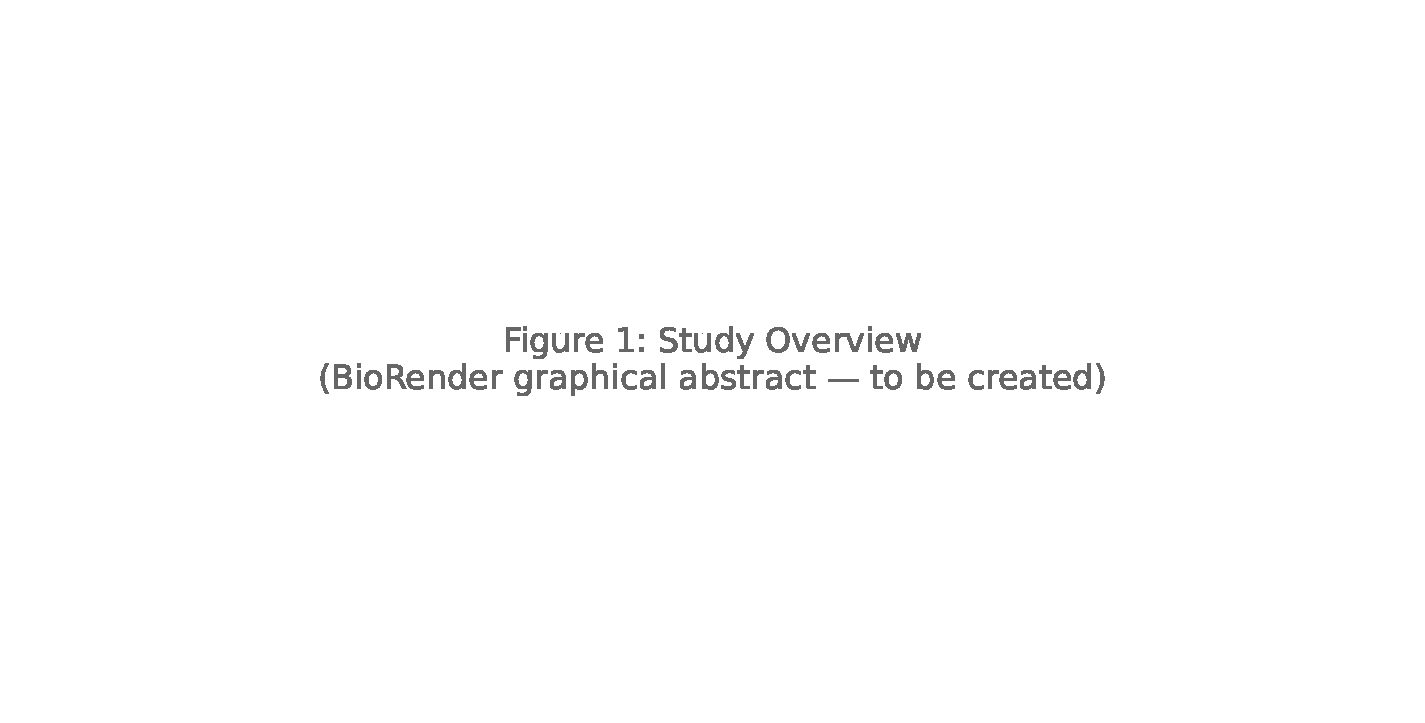
\includegraphics[width=\linewidth]{fig1_overview}
  \caption{\textbf{Study overview.}
    \textbf{(A)} Ten spaceflight radiation-response genes spanning four functional
    categories: DNA damage response (BRCA1, TP53, CHEK2, ATM, RAD51), epigenetic
    regulation (DNMT3A), telomere maintenance (TERT), oxidative stress response
    (NFE2L2), circadian rhythm (CLOCK), and muscle homeostasis (MSTN).
    \textbf{(B)} Evo2 scoring pipeline: for each variant, the reference and
    alternate sequences are scored within an 8,192\,\bp{} window centred on the
    variant; the log-likelihood difference ($\Delta$LL) quantifies predicted
    deleteriousness.
    \textbf{(C)} Three-layer validation: deep mutational scanning (DMS) calibration
    $\to$ ClinVar clinical benchmarking $\to$ non-coding functional validation
    (TERT MPRA, ENCODE cCREs).}
  \label{fig:overview}
\end{figure}

\begin{figure}[p]
  \centering
  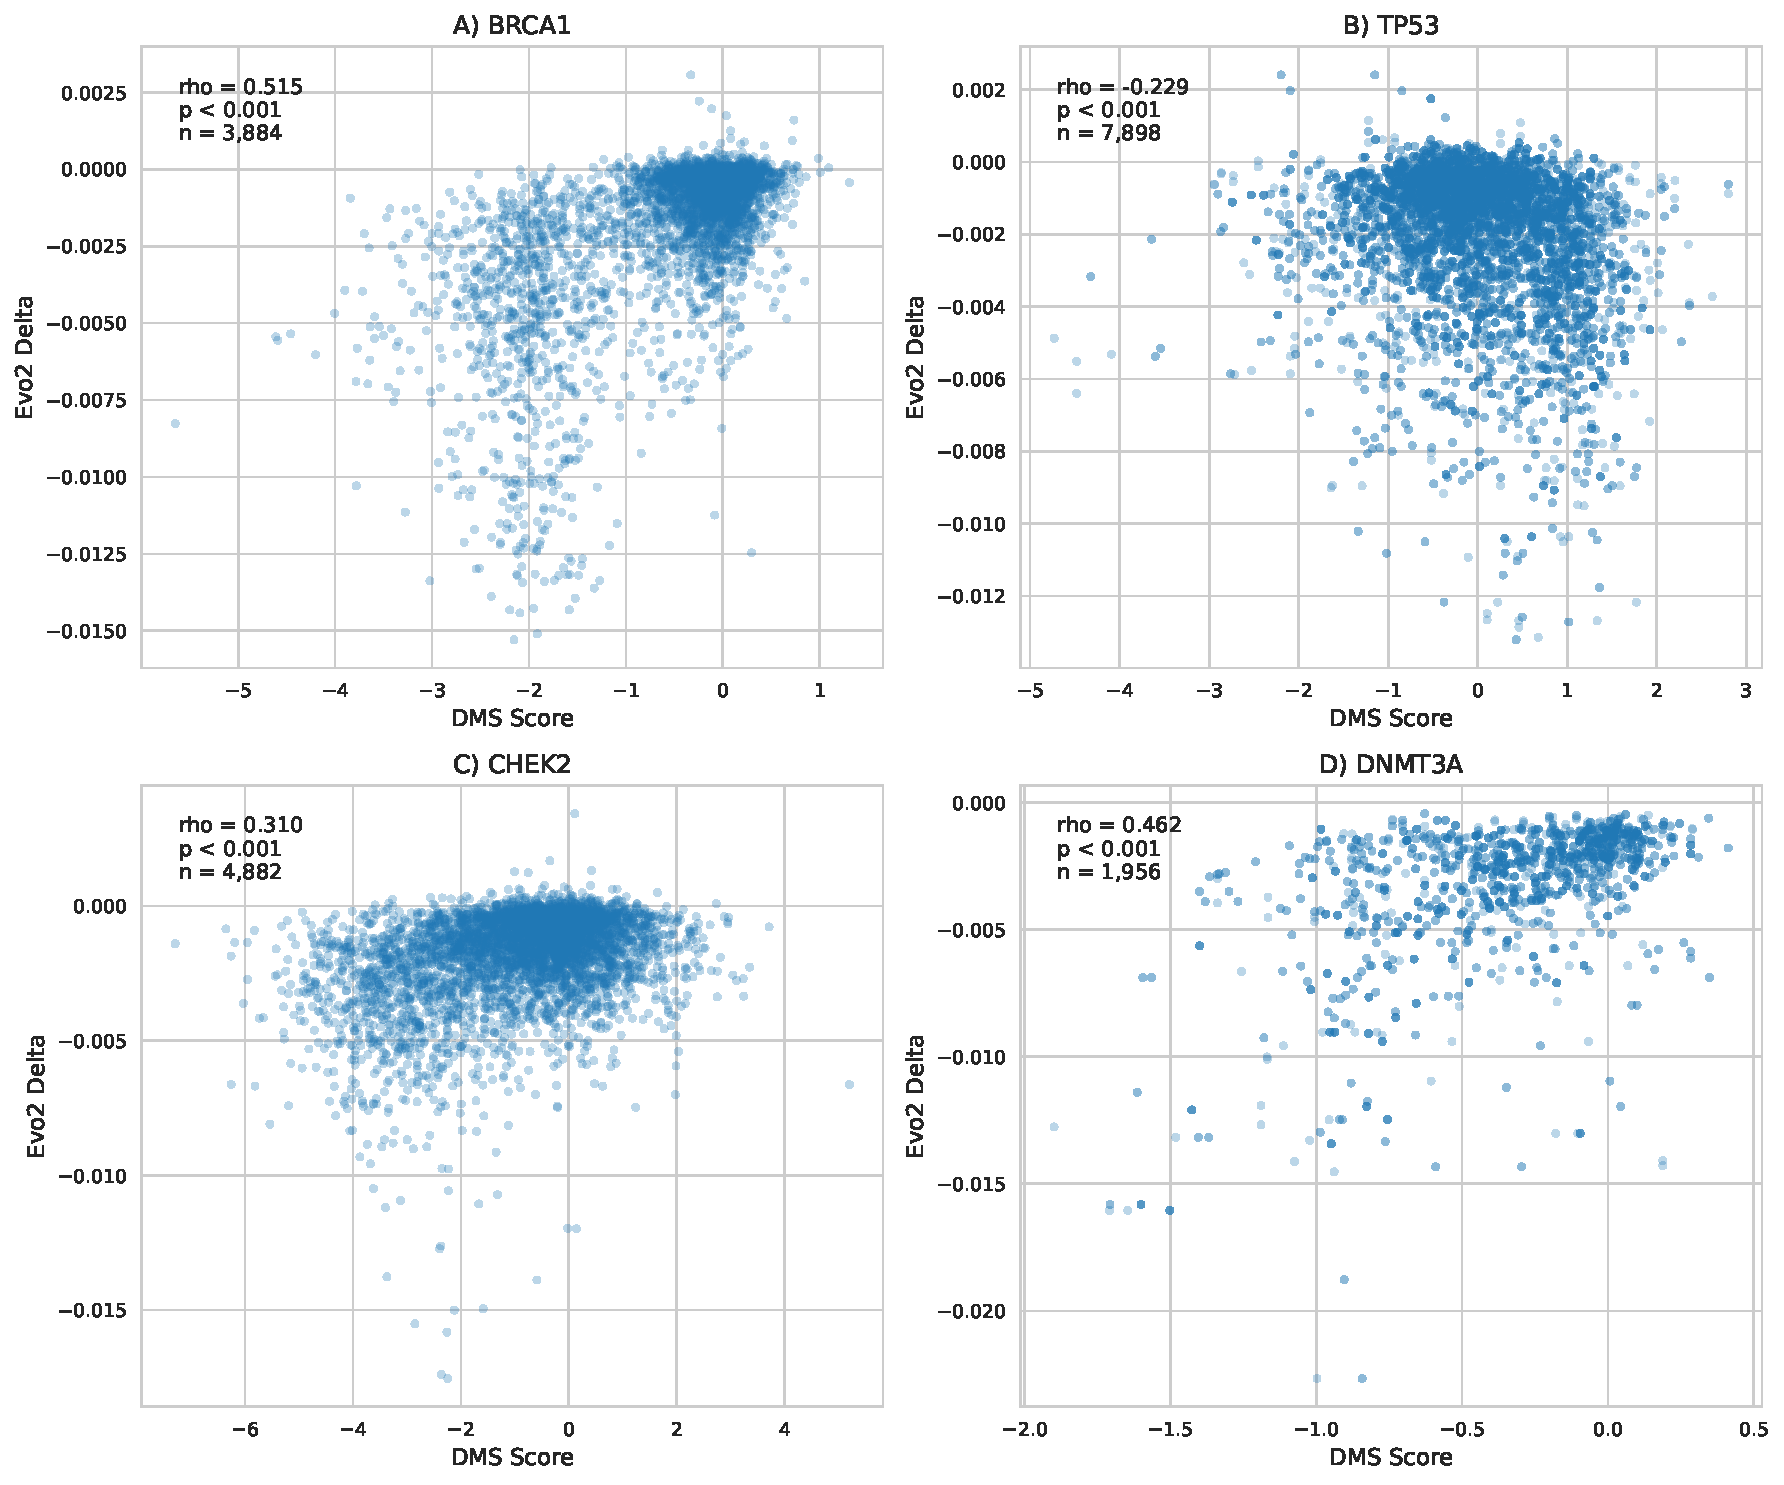
\includegraphics[width=\linewidth]{fig2_dms}
  \caption{\textbf{DMS calibration of Evo2 scores.}
    \textbf{(A--D)} Scatter plots of Evo2 $\Delta$LL vs.\ DMS functional score
    for BRCA1 (Findlay SGE, $\rho = +0.515$, $n = 3{,}884$),
    DNMT3A (Garcia paired fitness, $\rho = +0.457$, $n = 746$),
    CHEK2 (McCarthy-Leo abundance, $\rho = +0.310$, $n = 4{,}882$),
    and TP53 (Giacomelli nutlin-3, $\rho = -0.211$, $n = 2{,}827$;
    sign reflects LOF assay polarity).
    \textbf{(E)} Multi-tool comparison of $|\rho|$ with DMS scores on the
    same variant sets: Evo2 vs.\ AlphaMissense, CADD, REVEL, SpliceAI, and ncER.}
  \label{fig:dms}
\end{figure}

\begin{figure}[p]
  \centering
  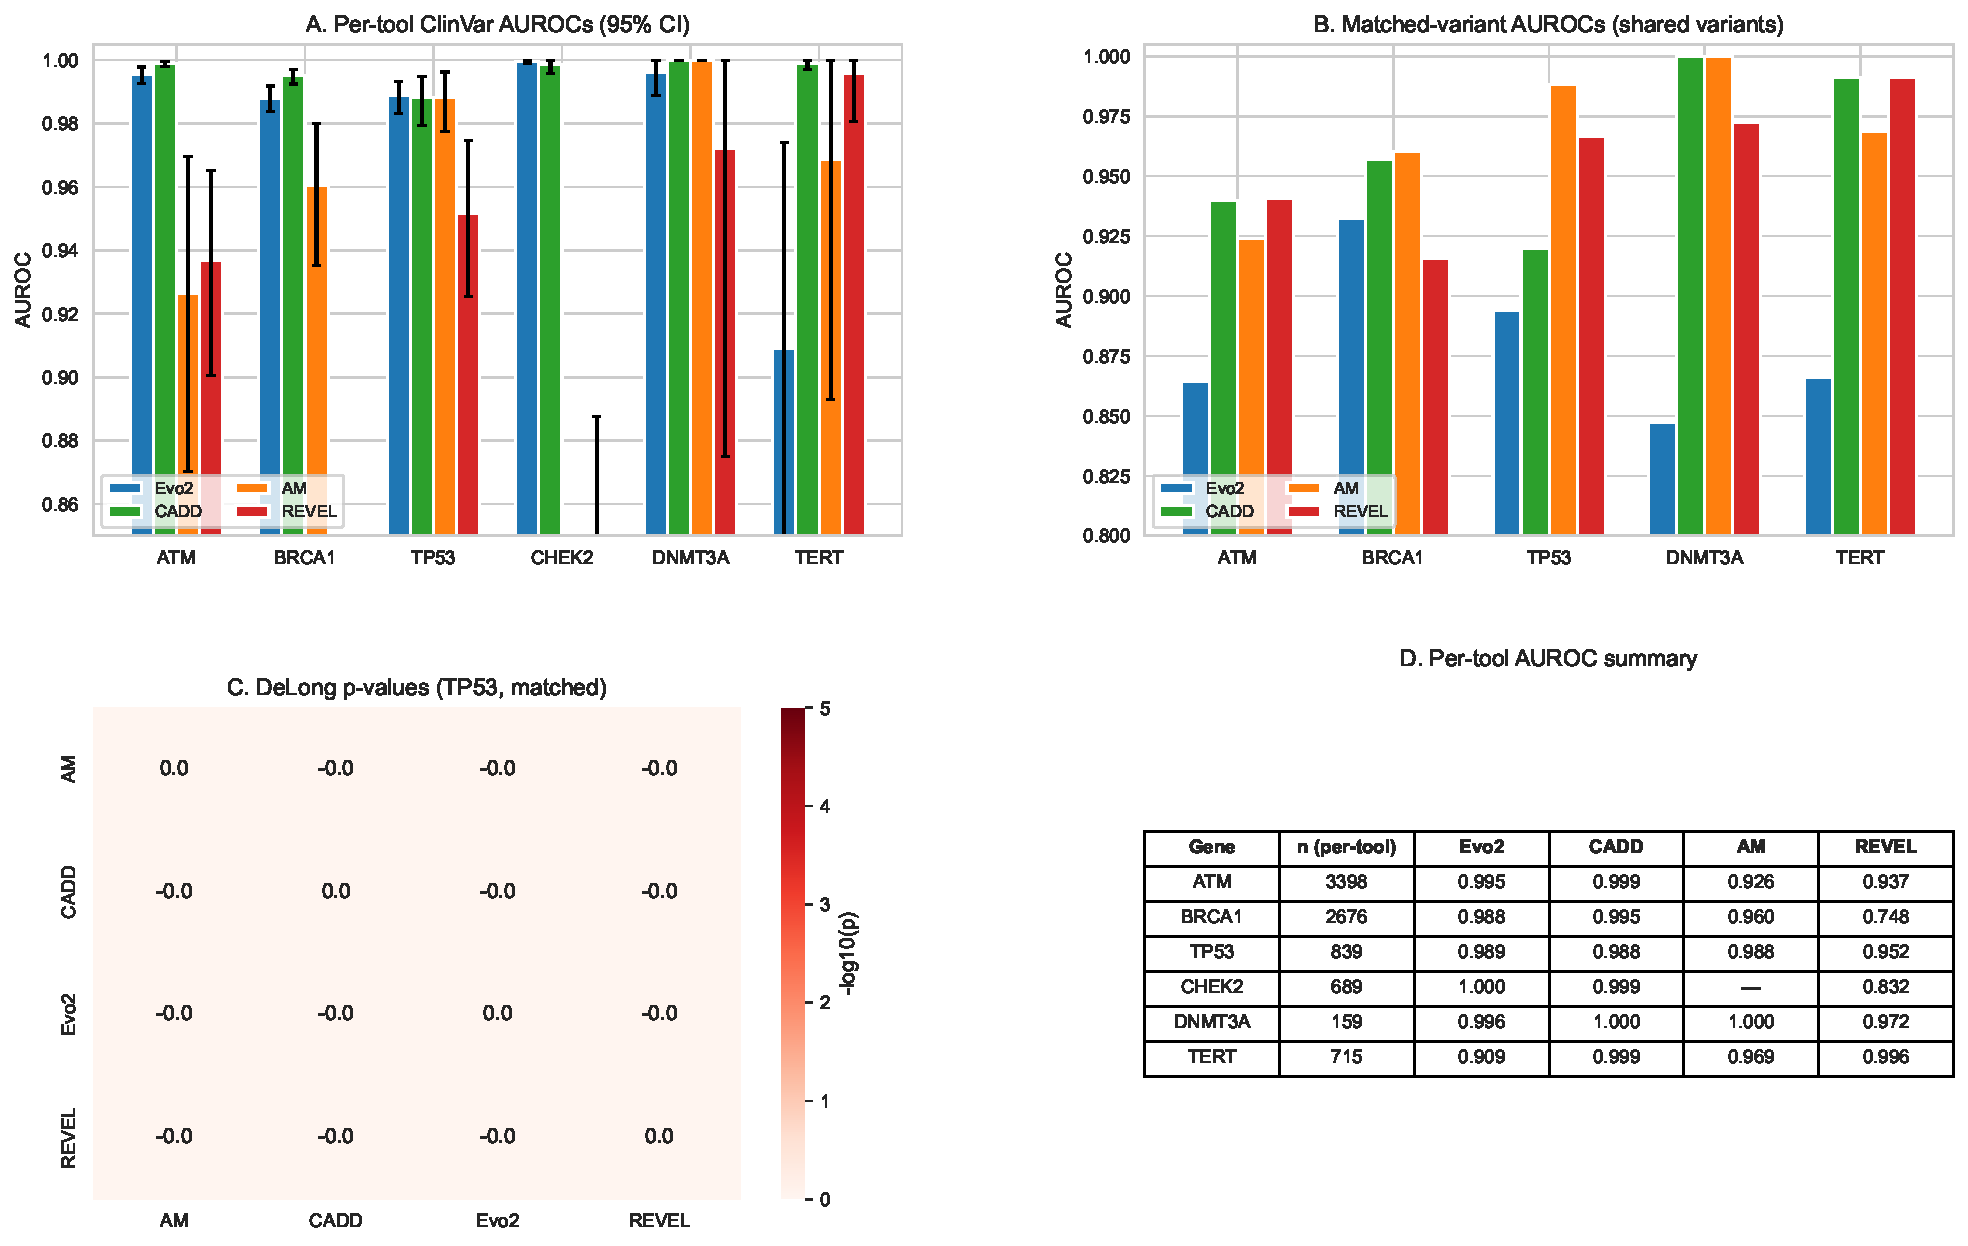
\includegraphics[width=\linewidth]{fig3_clinvar}
  \caption{\textbf{ClinVar clinical validation.}
    \textbf{(A)} ROC curves for Evo2 across six genes with sufficient
    pathogenic/benign ClinVar variants ($\geq$2-star review status).
    \textbf{(B)} Per-tool AUROCs with 95\% bootstrap confidence intervals
    (1,000 iterations) for Evo2, CADD, AlphaMissense, and REVEL.
    \textbf{(C)} Matched-variant AUROCs (intersection of variants scored by
    all four tools), providing a head-to-head comparison on identical variant sets.
    \textbf{(D)} DeLong test $p$-value matrix for pairwise AUROC differences
    on matched sets.}
  \label{fig:clinvar}
\end{figure}

\begin{figure}[p]
  \centering
  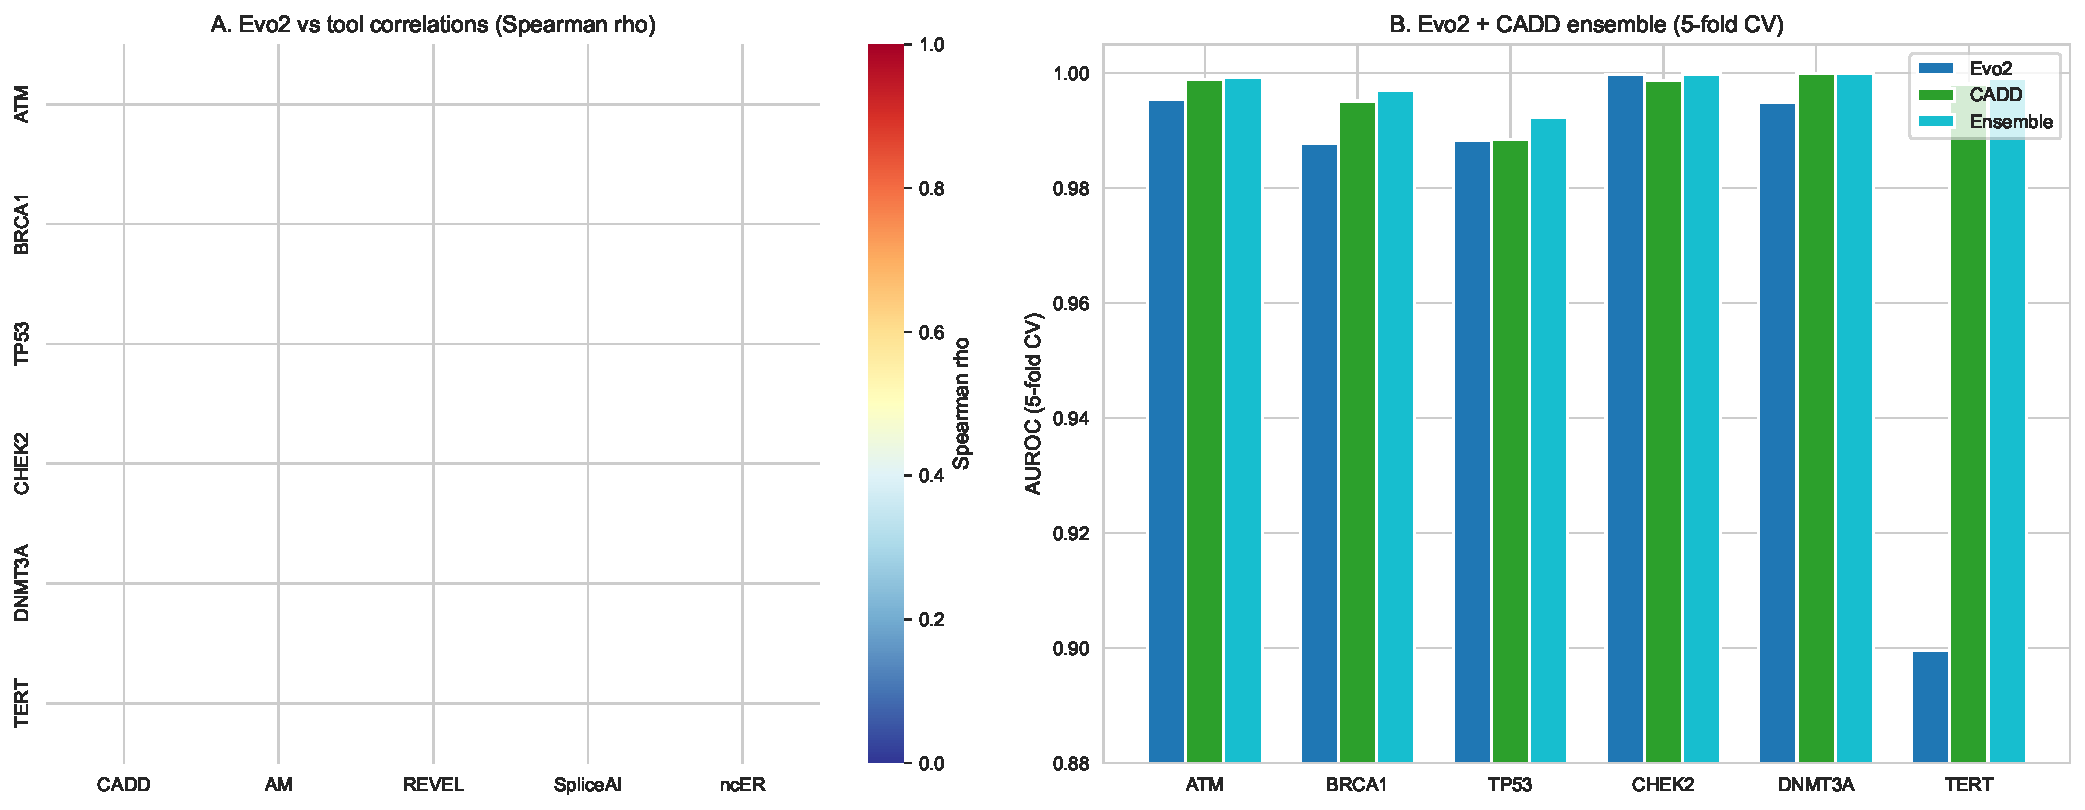
\includegraphics[width=\linewidth]{fig4_orthogonality}
  \caption{\textbf{Orthogonality and ensemble performance.}
    \textbf{(A)} Pairwise Spearman correlation heatmap between Evo2 and
    supervised tools across six genes, demonstrating complementary signal
    (Evo2 vs.\ CADD: $\rho = 0.41$--$0.83$; vs.\ SpliceAI: $\rho = 0.05$--$0.45$).
    \textbf{(B)} Five-fold cross-validated AUROC for Evo2-only, CADD-only,
    and logistic-regression ensemble (Evo2 + CADD); ensemble always $\geq$
    best single tool, with TP53 showing the largest gain ($+0.38\%$).}
  \label{fig:orthogonality}
\end{figure}

\begin{figure}[p]
  \centering
  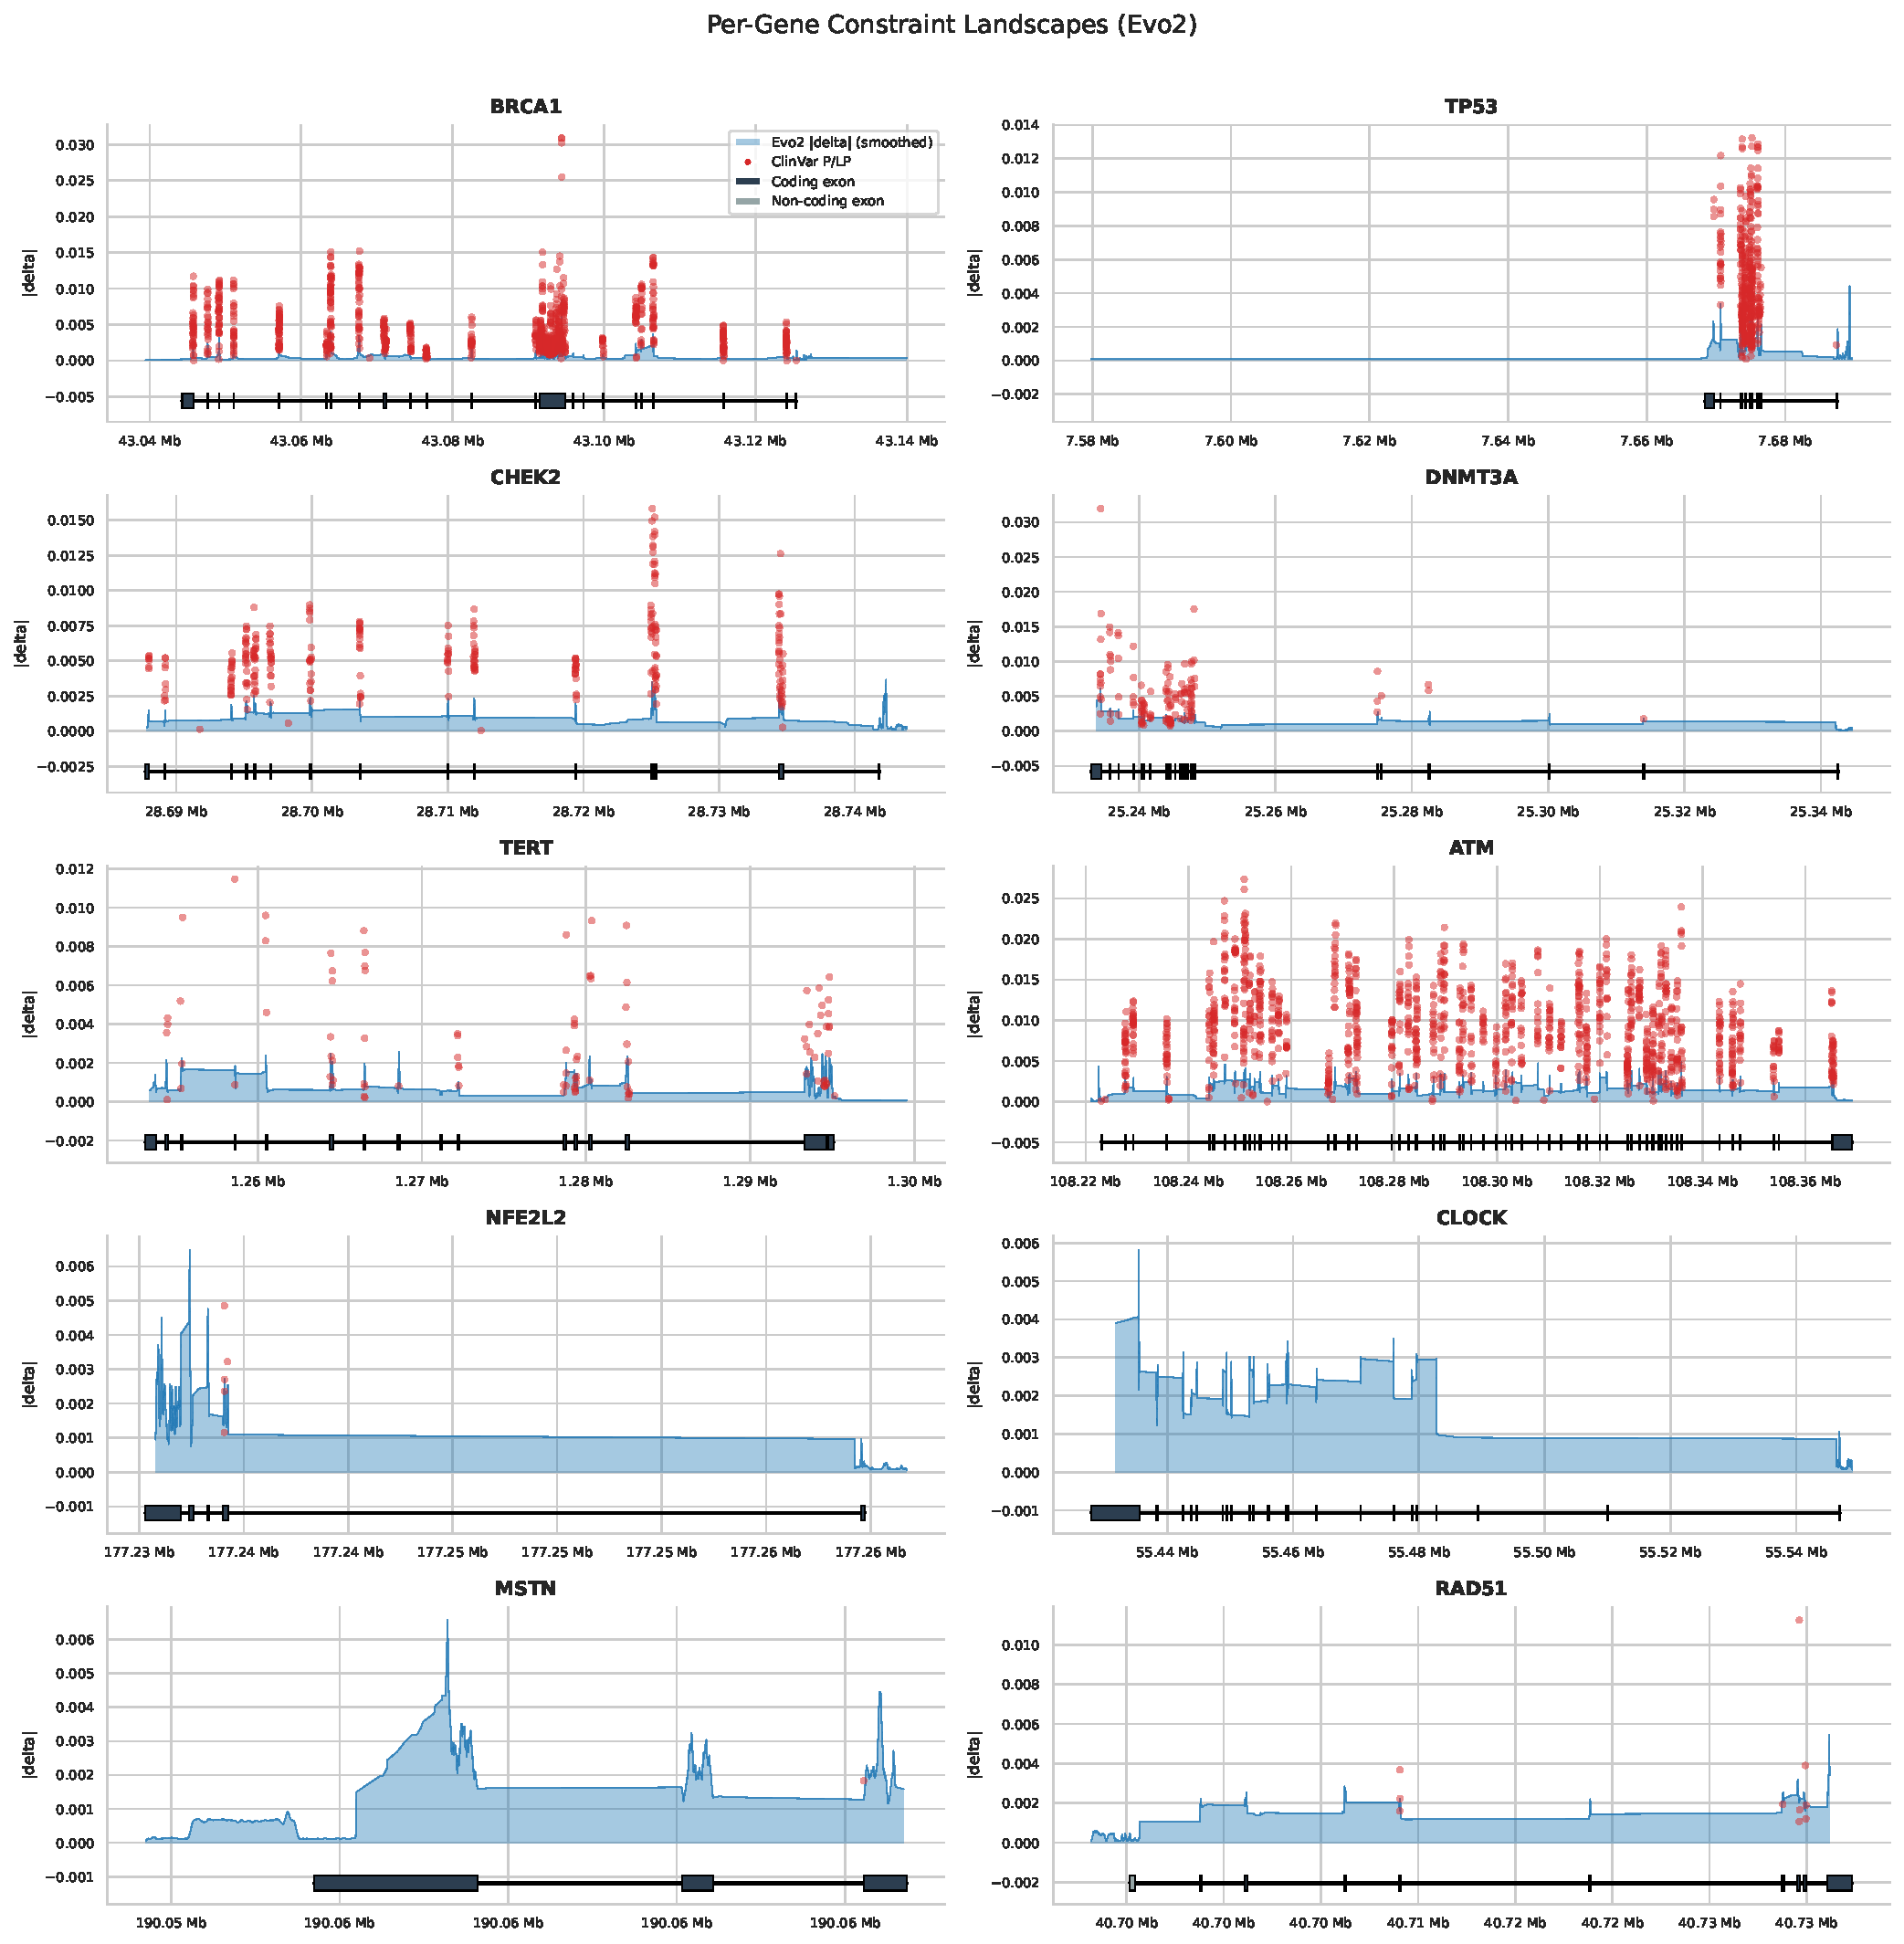
\includegraphics[width=\linewidth]{fig5_landscapes}
  \caption{\textbf{Gene-level variant effect landscapes.}
    Evo2 $\Delta$LL profiles across the ten gene loci. Exons are shaded;
    known protein domains (kinase, RING, BRCT, MTase, etc.)\ are annotated.
    Variants are plotted as smoothed score densities along the genomic
    coordinate. Functional domain boundaries correspond to regions of
    elevated predicted deleteriousness.}
  \label{fig:landscapes}
\end{figure}

\begin{figure}[p]
  \centering
  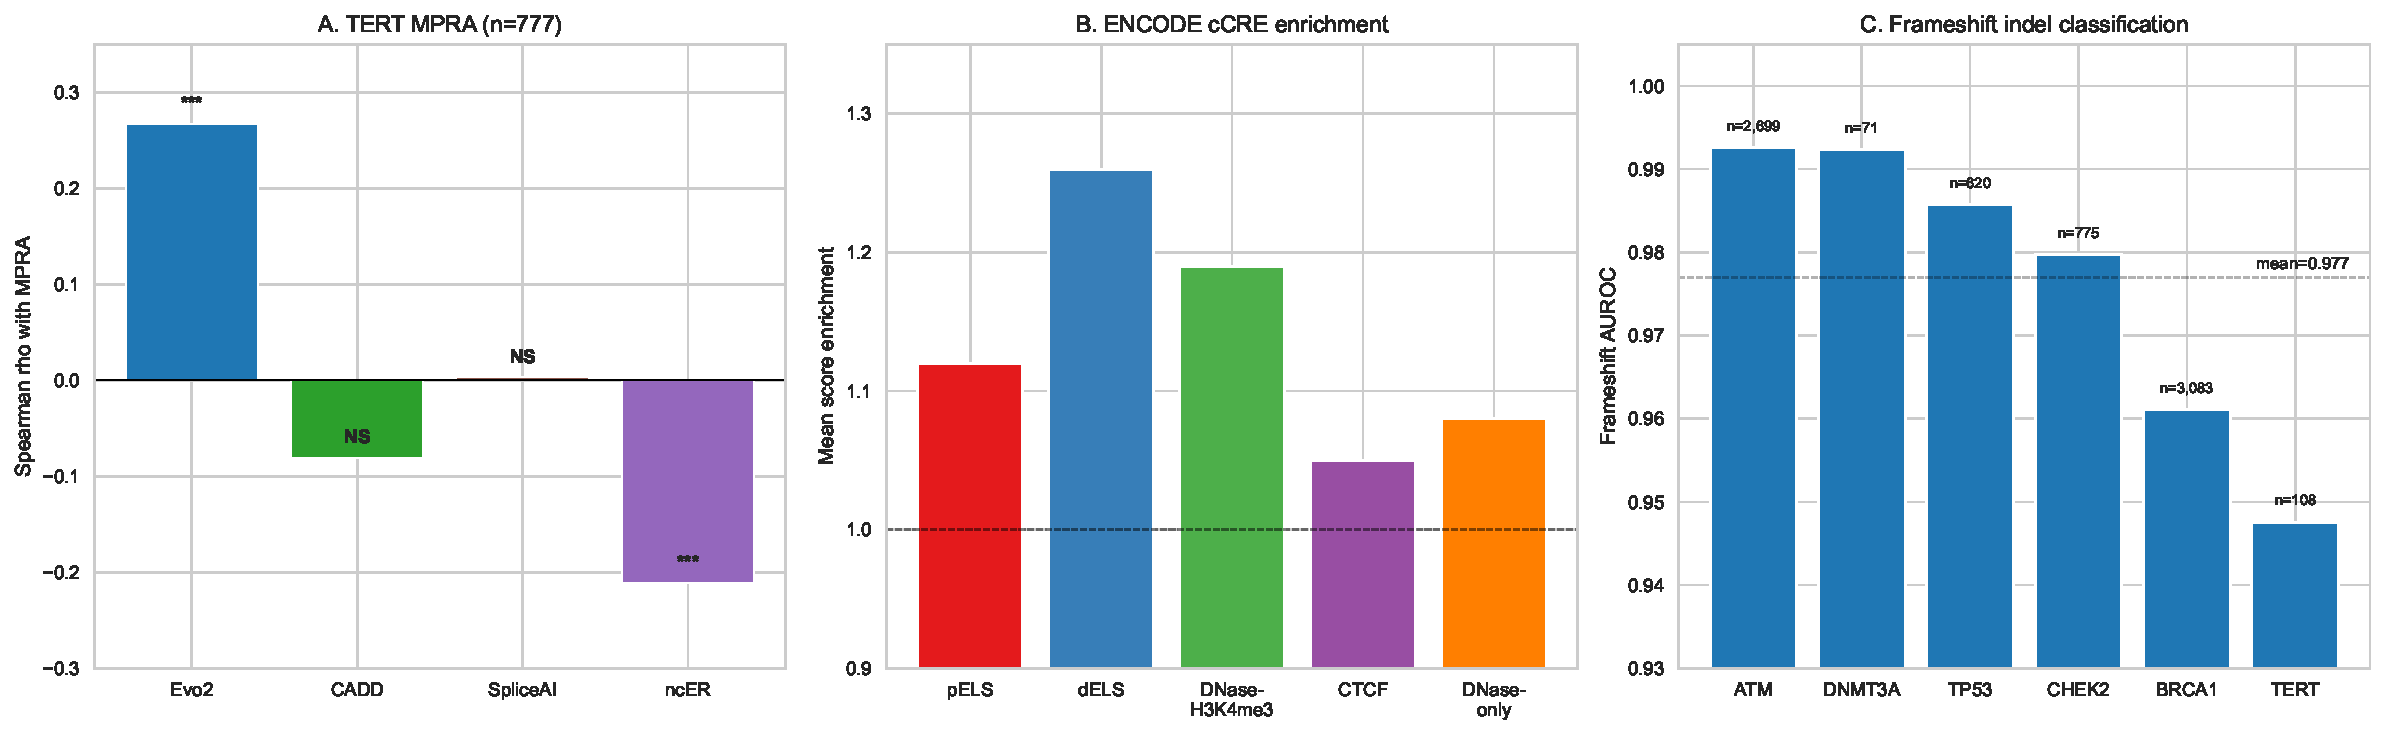
\includegraphics[width=\linewidth]{fig6_noncoding_indels}
  \caption{\textbf{Non-coding validation and indel scoring.}
    \textbf{(A)} TERT promoter MPRA: Evo2 $\Delta$LL vs.\ GBM reporter
    activity (Spearman $\rho = +0.267$, $p = 3.8 \times 10^{-14}$, $n = 777$);
    multi-tool comparison shows Evo2 is the only tool with a significant
    positive MPRA correlation (CADD: $\rho = -0.081$, NS; SpliceAI: $\rho = +0.003$, NS).
    \textbf{(B)} ENCODE cCRE enrichment analysis: variants in distal enhancer-like
    signatures (dELS) and proximal enhancer-like signatures (pELS) show elevated
    Evo2 scores relative to non-cCRE variants.
    \textbf{(C)} Frameshift indel classification: ClinVar P/LP vs.\ B/LB AUROC
    for six genes (mean $= 0.977$, range $0.948$--$0.993$).}
  \label{fig:noncoding}
\end{figure}

% --- Bibliography ---
\bibliographystyle{unsrtnat}
\bibliography{references}

\end{document}
